\section{Using equations} 

The Cadillac Escalade is a cross between a sports utility vehicle (SUV) and luxury car.  Either way, it's a big car.  And it takes awhile to stop.  One study showed that the 2010 Escalade traveling at 60 miles per hour takes about 144 feet to come to a complete stop from when the driver first hits the brakes.   In fact, the braking distance of any car depends on how fast it is going.  If someone is driving slowly they can stop in shorter distance than if they are driving fast.  Which is why you should drive slowly on residential streets.  

We would like to be able to calculate the braking distances at other speeds, so our two variables are
\begin{center}
\begin{tabular} {l} 
$S=$ speed (mph) $\sim$ indep \\
$B= $ braking distance (feet) $\sim$ dep \\ 
\end{tabular}
\end{center}
Using the data and equations from physics, automobile analysts were able to determine that the equation relating these two variables is $$B=.04S^2$$  Remember that the .04 written next to the $S^2$ means they are multiplied.  We might equally well have written $$B = .04 \ast S^2$$ 

You may be a little surprised to see the variable $S$ \textbf{squared} (raised to the 2nd power) or wonder what the number .04 means.  This equation is not something we can figure out because it relies both on the data and knowledge of the physics involved.  But, we can still work with this equation to find the braking distances at any speed.   (If you must know, this equation is only approximate since things like tire and road conditions are a factor, but for what we want it is good enough.)

Although in the last couple of sections we were able to find equations by generalizing examples, there are actually many different mathematical and statistical techniques for finding equations. A scientist might use lab experiments and some theory to figure it out.  An economist might recognize that the equation fits a certain template because of the underlying economics.  A store manager might know from years of experience that a certain equation works well to predict sales.  It can be comforting to know where an equation comes from but whether we find an equation for ourselves or get it from an expert, we can use it to answer our questions and make predictions. 

Now that we have an equation we can calculate the braking distance for a Cadillac Escalade traveling 30, 50, 70 or 90 miles per hour.  For 30 miles per hour, we have $S=30$.  So, we substitute 30 in place of the $S$ in the equation to get 
$$B = .04 \ast 30^2 = .04\times \underline{30} \wedge 2 = 36 \text{ feet}$$  
At 30 mph, it takes the Cadillac Escalade 36 feet to stop.  As we expected, it doesn't take nearly as far to stop as it did at 60 mph. 
Quick bit of terminology.  When we know the independent variable, like $S=30$ and we substitute into the equation to find the dependent variable, like $B=36$, we say we \textbf{evaluate} the function $B$ at $S=30$.

For the other speeds we do the same thing:  evaluate at the appropriate value of  $S$.  When  $S=50$ mph we get
$$B = .04 \ast 50^2 = .04\times \underline{50}\wedge2 = 100 \text{ feet}$$ 
When $S=70$ mph we get
$$B = .04 \ast 70^2 = .04\times \underline{70}\wedge2 = 196\text{ feet}$$ 
When $S=90$ mph we get
$$B = .04 \ast 90^2 = .04\times \underline{90}\wedge2 = 324 \text{ feet}$$ 
And, what does our equation tell us when the speed is 0 mph?  We evaluate at $S=0$ mph to get  $$B = .04 \ast 0^2 = .04\times \underline{0} \wedge 2 = 0 \text{ feet}$$ 
Well, sure!  If the car isn't moving, then it won't need any distance to stop.
Here's what we've found so far, displayed in a table.
\begin{center}
\begin{tabular} {|c| |c|c |c|c|c |c|} \hline
$S$ & 0 & 30 & 50 & 60 & 70 & 90 \\ \hline
$B$ & 0 & 36 & 100 & 144 & 196 & 324 \\ \hline
\end{tabular}
\end{center}

My neighbor Jeff happens to drive a 2010 Cadillac Escalade.  The other day he almost was in an accident on the highway.  Luckily no one was hurt, but he had to slam on the brakes to stop.  The police report mentioned they believe it took his car 183 feet to stop.  Jeff says he was not driving over the posted speed limit of 65 mph.  Should we believe him?

We can see from the table that braking distance of 183 feet falls in between the 144 and 196 on our table which leads us to believe that Jeff was traveling faster than 60 mph and slower than 70 mph.  We can figure out if Jeff were driving at 65 mph, then his braking distance would have been 
$$B = .04 \ast 65^2 = .04\times \underline{65} \wedge 2 = 169 \text{ feet}$$  That's less than the 183 feet Jeff took to stop.  So, it appears that Jeff was driving faster than 65 mph. 

But wait a minute.  The braking distance is just the time it takes from when the driver's foot hits the brake until the car stops.  That distance doesn't take into account the driver's reaction time -- how long between when the driver thinks to stop and when the driver's foot actually hits the brake.  We have a new dependent variable
\begin{center}
\begin{tabular} {l} 
$D=$ total stopping distance (feet) $\sim$ dep \\ 
$S=$ speed (mph) $\sim$ indep \quad \emph{as before}\\
\end{tabular}
\end{center}

How can we include this reaction time into an equation?  Suppose it takes 1 second to react.  We would like to know how many feet that adds to the equation.  This is something we can figure out.  We know the speed and the time, so multiply them to get the distance, right?  One small snag:  the speed is in mph (miles per hour).  We need to convert units.    
$$1 \text{ \cancel{sec}} \ast \frac{1 \text{ \cancel{min}}}{60 \text{ \cancel{sec}}} \ast \frac{1 \text{ hour}}{60 \text{ \cancel{min}}} \ast \frac{\text{5,280 feet}}{1 \text{ mile}}=1 \div 60 \div 60 \times \text{5,280}= 1.4666\ldots \approx 1.47 \text{ feet per mph}$$
added to the stopping distance. 
Notice the fancy fraction work  with the units?
$$\frac{\text{hour}\ast \text{feet}}{\text{mile}}=\frac{\text{feet}}{\quad \frac{\text{miles}}{\text{hour}}\quad~}=\frac{\text{feet}}{\text{mph}}$$
What all this mess means is that we should add 1.47 feet for every mph of speed.  
So $S$ mph adds $1.47\ast S$ feet to the stopping distance.
 Long story short, our new equation is
 $$D=.04S^2+1.47S$$

Something interesting about this equation. The independent variable $S$ appears twice; first for the braking distance and again because of the reaction time. When we evaluate the equation we need to plug in the value of $S$ in two places.  Check it out.
When $S=30$ mph we have $$D =  .04 \ast  30^2 + 1.47 \ast 30 = .04\times \underline{30} \wedge 2 +1.47 \times \underline{30} = 80.10 \approx 80 \text{ feet}$$ 
That's a lot further than just the braking distance of 36 feet.
When $S=50$ mph we have $$D = .04 \ast  50^2 +1.47\ast 50 =  .04\times \underline{50} \wedge 2 +1.47\times \underline{50} = 173.50 \approx 174 \text{ feet}$$
again, much more than the braking distance of 100 feet.
Here's the revised table of values.
\begin{center}
\begin{tabular} {|c| |c|c |c|c|c |c|} \hline
$S$ & 0 & 30 & 50 & 60 & 70 & 90 \\ \hline
$D$ & 0 & 80 & 174 & 232 & 299 & 456 \\ \hline
\end{tabular}
\end{center}

These numbers make us rethink Jeff's assertion.  Given that he stopped in 183 feet, which is much less than the 232 feet it takes to stop at 60 mph, it looks like Jeff was driving less than 60 mph.  To be sure, calculate that at 65 mph, it would have taken Jeff
 $$D = .04 \ast  65^2 + 1.47 \ast  65  = .04\times \underline{65} \wedge 2+ 1.47\times \underline{65} =264.55 \approx 265 \text{ feet}$$  Again, we should believe Jeff.  And, be glad nobody was hurt.

A quick glance at the graph confirms our findings.  
\begin{center}
\scalebox {.8} {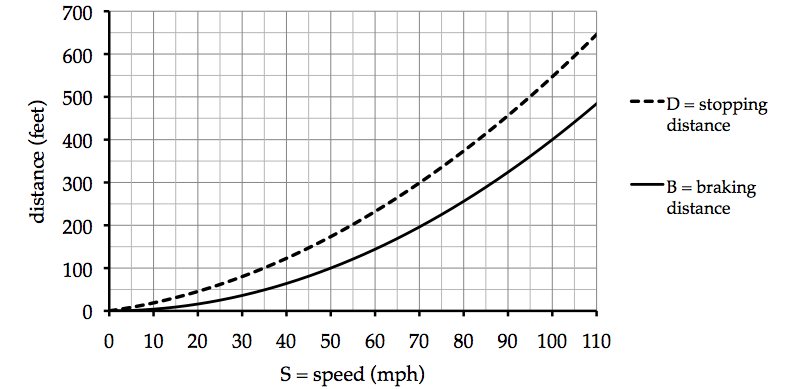
\includegraphics [width=7in] {cadillacBRAKESTOP.png}}
\end{center}
The distance of 183 feet falls just above the unlabeled gridline for 175 and below the gridline for 200.  Looking at the corresponding point on the braking distance curve, it looks like it falls around 67 mph, but looking at the corresponding point on the stopping distance curve, it looks like just over 50 mph.
% SU the exact values happen to be 67.638... and 51.715...  Return to that in 3.5 solving quads

By the way, our first equation $$B = .04 \ast S^2$$ is a \textbf{power equation} because the independent variable is being raised to a power, $n=2$, and then scaled by a \textbf{proportionality constant}, $k=.04$.  Any power equation fits this template.

\bigskip
 \framebox{
 \begin{minipage}[c]{.85\textwidth}  
~ \bigskip \\  \textsc{Power equation template:} \quad $\text{dep} = k \ast \text{indep}^{n}$\\ ~ \bigskip
\end{minipage}
}
\bigskip

\noindent Our second equation  $$D=.04S^2 + 1.47S$$ is a \textbf{polynomial equation} because includes a sum of linear and powers.  The exercises introduce more polynomial equations.  
SU LIST HERE???
In our equation, the highest power of the independent variable happens to be 2 (squared).  This type of polynomial equation has a special name.  It is a \textbf{quadratic equation}.  Any quadratic equation fits this template.

\bigskip
 \framebox{
 \begin{minipage}[c]{.85\textwidth}  
~ \bigskip \\  \textsc{Quadratic equation template:} \quad $\text{dep} = a \ast \text{indep}^2 + b \ast\text{indep} + c$\\ ~ \bigskip
\end{minipage}
}
\bigskip

\noindent For our equation $a=.04$, $b=1.47$, and the mysteriously missing $c=0$.  Much more on that later.  


SU -- what section does this belong in:

\begin{quote}
Evaluating uses the usual order of operations:
\begin{enumerate}
\item Parentheses
\item Powers (and roots and logs)
\item Multiplication and division
\item Addition and subtraction
\end{enumerate}
\end{quote}%Su cite?

%\newpage

%%\section{Using equations} 

 \begin{center}
\line(1,0){300} %\line(1,0){250}
\end{center}

\section*{Homework}

\noindent \textbf{Start by doing Practice exercises \#1-4 in the workbook.}

\bigskip
 
\noindent \textbf{Do you know \ldots}

\begin{itemize}
\item What it means to ``evaluate'' a function? 
\item Why some numbers are underlined in our calculation?
\item How to evaluate an function when the independent variable occurs more than once? 
\item How to generate a table or graph from an equation? 
\item What graphs of different types of functions look like? 
\item What a power, polynomial, or quadratic equation look like?
\item[~] \textbf{If you're not sure, work the rest of exercises and then return to these questions.  Or, ask your instructor or a classmate for help.} 
\end{itemize} 

\subsection*{Exercises}

\begin{enumerate} 
\setcounter{enumi}{4}

\item The 2002 Chevrolet Tahoe 4WD will take about 158.1 feet to stop when traveling at 60 mph in normal highway conditions.  Let $S$ be the speed at which the vehicle is traveling, in miles per hour (mph), and $D$ the distance it takes to stop, in feet.  This information together with a little physics gives the equation $$D = .0439S^2 + 1.47S$$
\begin{enumerate}
\item According to this equation, how many feet does it take to stop the Tahoe when traveling 80 miles per hour?
\item In driver's training classes they teach the ``two-second rule'' for safety:  you should follow no closer than two seconds behind the car in front of you.  If you are traveling 80 miles per hour, how many feet can you travel in two seconds?  \emph{Hint: convert to feet per second, then multiply by two seconds.}
\item Compare your results from parts (a) and (b) to decide if the ``two-second rule'' is adequate for safety at 80 miles per hour.  That is, if you are following two seconds behind the car in front of you and calamity strikes that car, will you be able to stop before hitting it?
\item Is the ``two-second rule'' adequate at 50 mph?
\end{enumerate}

\item Mom always said to sit close to the lamp when I was reading.  The intensity of light $L$, measured in percentage (\%) that you see from a lamp depends on your distance from the lamp, $F$ feet as described by the formula $$L=\frac{100}{F^2}$$
 \hfill \emph{Story also appears in 1.1 and 3.3 Exercises}
\begin{enumerate}
\item Calculate the  intensity when I sit 1 foot, 2 feet, or 3 feet away.
\item The other day I was sitting 27 inches from the lamp. What was the intensity of the light there? 
\item Calculate the rate of change of light intensity between 2 feet and 27 inches.  What does that tell you in terms of the story?
\item Draw a graph illustrating the function.
\end{enumerate}

\item Urban community gardens are catching on.  What was once an abandoned lot down the block is now a thriving 10'$\times$25' vegetable and berry garden for the neighborhood. (Remember ' stands for ``feet,'' so the garden is 10 feet wide and 25 feet long.)  One neighbor volunteered to donate gravel to make a path around the garden.  The path will be 3 inches deep and the same width all around. 
\begin{center}
\scalebox {.4} {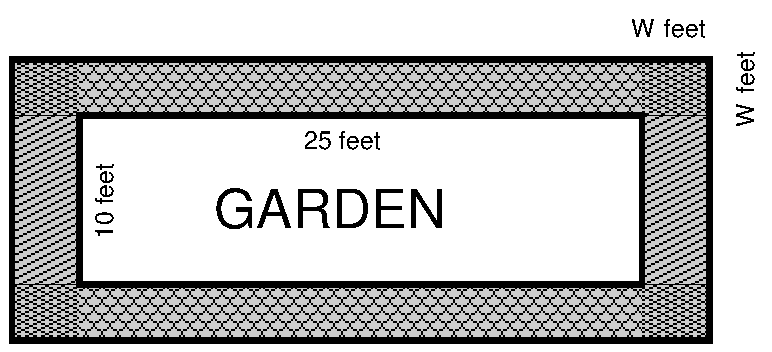
\includegraphics{GravelPath.pdf}}
\end{center}
 \hfill \emph{Story also appears in 2.4 Exercises and 3.5 \#4}
\begin{enumerate}
\item The other measurements are in feet, so convert the depth of the path (3 inches) into feet also.  
\item Suppose for the moment that the path will be 4 feet wide. Calculate the area of the path.  Here's one way to do it:  first, find the area of the outer rectangle, then subtract the area of the garden itself.

\emph{Hint:  the length of that outer rectangle includes the 25 feet of garden plus the width of the path on each side.   Same for the width of that outer rectangle.}
\item Figure out how much gravel they would need  (in cubic feet) for a 4 foot wide path by multiplying your answers to (a) and (b). 
\item  Actually, they aren't sure how wide the path should be and how much gravel they can get.  Let's write $W$ = width of path (feet) and $G$ = amount of gravel (cubic feet).  It turns out that $$G = W^2 + 17.5W$$
Check that when you evaluate at $W=4$ you get the same answer as in (c).
\item How many cubic feet of gravel would they need to make the path 2 feet wide? 3 feet wide?  42 inches? 
\end{enumerate}

\item One measure of the diversity of our news source is the count of the number of different daily newspapers in circulation.  A reasonable equation estimating this count over the past century is $$N = -.0021T^3+.34T^2-20T+ \text{2,226}$$ where $N$ is the number of daily newspapers in circulation in the United States $T$ years after 1900.
\begin{enumerate}
\item Based on this equation, how many daily newspapers were in circulation in 1920?  In 1955?  In 1995?  In 2010?
\item During which period were the number of newspapers in circulation dropping faster:  1900 to 1920 or 1995 to 2010?
\item Draw a graph illustrating the dependence.
\end{enumerate}

\item Mrs.\ Weber's cooking class came up with the equation $$M = 1.2F^2+4F+7$$ to approximate the grilling time of a piece of fish depending on its thickness.  Here $M$ is the number of minutes to grill the fish and $F$ is the thickness of the fish (in inches).  

\hfill \emph{Story also appears in 1.1 and 3.5 Exercises}
\begin{enumerate}
\item Evaluate the equation at $F=.25, 1, 1.5,$ and $2$.
\item What do the answers you found say about cooking fish?
\item Draw a graph showing how the cooking time depends on the thickness of the fish.
\item Your graph should show that the function is increasing.  Explain how that makes sense in terms of the story.
\end{enumerate} 

\item Wynter has a pretty decent job. He is paid a salary of \$780 per week but his hours vary week-to-week. Even though Wynter is not paid by the hour, he can figure out what his hourly wage would be depending on the number of hours he works.  For example, in a week where Wynter works 40 hours, he's earning the equivalent of \$19.50/hr because $$\frac{\$780}{40 \text{ hours}} = 780 \div 40 =\$19.50\text{/hour}$$

\hfill \emph{Story also appears in 3.3 Exercises}
\begin{enumerate}
\item What's Wynter's equivalent hourly wage in a week when he works 50 hours? 60 hours?
\item Name the variables and write an equation relating them.
\item Explain why this function is decreasing.
\end{enumerate} 


\end{enumerate}
